\documentclass[12pt]{article}
\usepackage[left=0.25cm,top=1cm,right=0.25cm,bottom=1cm]{geometry}
\textwidth = 20cm
\hoffset = -1cm
\usepackage[utf8]{inputenc}
\usepackage[spanish,es-tabla]{babel}
\usepackage[autostyle,spanish=mexican]{csquotes}
\usepackage[tbtags]{amsmath}
\usepackage{nccmath}
\usepackage{amsthm}
\usepackage{amssymb}
\usepackage{graphicx}
\usepackage{standalone}
\usepackage[outdir=./]{epstopdf}
\usepackage{siunitx}
\usepackage{physics}
\usepackage{color}
\usepackage{float}
\usepackage{multicol}
%\usepackage{milista}
\usepackage{enumitem}
\usepackage{anyfontsize}
\usepackage{anysize}
\usepackage{enumitem}
\usepackage{capt-of}
\usepackage{bm}
\usepackage{relsize}
\usepackage{placeins}
\usepackage{empheq}
\usepackage{cancel}
\usepackage{wrapfig}
\spanishdecimal{.}
\renewcommand{\baselinestretch}{1.5} 
\renewcommand\labelenumii{\theenumi.{\arabic{enumii}}}
\newcommand{\ptilde}[1]{\ensuremath{{#1}^{\prime}}}
\newcommand{\stilde}[1]{\ensuremath{{#1}^{\prime \prime}}}
\newcommand{\ttilde}[1]{\ensuremath{{#1}^{\prime \prime \prime}}}
\newcommand{\ntilde}[2]{\ensuremath{{#1}^{(#2)}}}


\title{Ls función de Green \\ \large {Tema 2 - Primeras técnicas de solución} \vspace{-3ex}}
\author{M. en C. Gustavo Contreras Mayén}
\date{ }

\pagestyle{fancy}
\fancyhf{}
\rhead{Curso MAF}
\lhead{\leftmark}
\rfoot{\thepage}
\setlength{\headheight}{16pt}%

\begin{document}
\vspace{-4cm}
\maketitle
\fontsize{14}{14}\selectfont
\tableofcontents
\newpage

%Ref. Herman (2015) - Green's functions and inhomogueneous equations
\section{Introducción.}

La ecuación de onda, la ecuación del calor y la ecuación de Laplace son ecuaciones diferenciales parciales homogéneas típicas. Se pueden escribir en la forma:
\begin{align*}
\mathcal{L} u (x) = 0
\end{align*}
donde $\mathcal{L}$ es un operador diferencial. Por ejemplo, estas ecuaciones se pueden escribir como:
\begin{align*}
\bigg( \pdv[2]{t} - c^{2} \, \laplacian \bigg) \, u &= 0 \\[0.25em]
\bigg( \pdv{t} - k \, \laplacian \bigg) \, u &= 0 \\[0.25em]
\laplacian{u} &= 0
\end{align*}

En este tema revisaremos soluciones de ecuaciones diferenciales parciales no homogéneas, del tipo:
\begin{align*}
\mathcal{L} u (x) = f (x)
\end{align*}
buscando la llamada función de Green. La historia de la función de Green se remonta a 1828, cuando George Green publicó un trabajo en el que buscaba soluciones de la ecuación de Poisson $\laplacian{u} = f$ para el potencial eléctrico $u$ definido dentro de un volumen acotado con condiciones de contorno específicas en la superficie del volumen. Introdujo una función ahora identificada como lo que Riemann más tarde acuñó como la \enquote{función de Green}. En esta parte obtendremos el valor inicial de la función de Green para ecuaciones diferenciales ordinarias. Más adelante en el capítulo volveremos a las funciones de Green de valor límite y a las funciones de Green para ecuaciones diferenciales parciales.
\par
Como un ejemplo simple, considere la ecuación de Poisson:
\begin{align*}
\laplacian{u} (\vb{r}) = f (\vb{r})
\end{align*}
Sea la ecuación de Poisson dentro de una región $\Omega$ limitada por la superficie $\partial \Omega$ como se muestra en la figura (\ref{fig:figura_07_01}). Esta es la forma no homogénea de la ecuación de Laplace. El término no homogéneo, $f (\vb{r})$, podría representar una fuente de calor en un problema de estado estacionario o una distribución de carga (fuente) en un problema electrostático.
\begin{figure}[H]
    \centering
    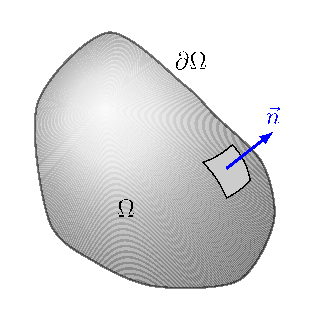
\includegraphics[scale=1]{Imagenes/Funcion_Green_01.eps}
    \caption{Consideremos la ecuación de Poisson dentro de una región $\Omega$ acotada por una superficie $\partial \Omega$}
    \label{fig:figura_07_01}
\end{figure}
Ahora pensemos en la fuente como una fuente puntual en la que estamos interesados en la respuesta del sistema a esta fuente puntual. Si la fuente puntual está ubicada en un punto $\vb{\pderivada{r}}$, entonces la respuesta a la fuente puntual podría sentirse en los puntos $\vb{r}$. Llamaremos a esta respuesta $G(\vb{r}, \vb{\pderivada{r}})$. La función de respuesta satisfaría una ecuación de fuente puntual de la forma:
\begin{align*}
\laplacian G(\vb{r}, \vb{\pderivada{r}}) = \delta (\vb{r} - \vb{\pderivada{r}})
\end{align*}
donde $\delta (\vb{r} - \vb{\pderivada{r}})$ es la función delta de Dirac. Una propiedad clave de esta función generalizada\footnote{Revisa el material de trabajo de la función delta de Dirac, en donde encontrarás varias propiedades, entre ellas, la propiedad de filtro.} es la propiedad de filtro:
\begin{align*}
\scaleint{6ex}_{\bs \Omega} \delta (\vb{r} - \vb{\pderivada{r}}) \, f (\vb{r}) \dd{V} = f (\vb{\pderivada{r}})
\end{align*}
La conexión entre la función de Green y la solución a la ecuación de Poisson se encuentra en la segunda identidad de Green:
\begin{align*}
\scaleint{6ex}_{\bs \partial \Omega} \bigg[ \phi \, \grad{\psi} - \psi \, \grad{\phi} \bigg] \cdot \vb{n} \dd{S} = \scaleint{6ex}_{\bs \Omega} \bigg[ \phi \, \laplacian{\psi} - \psi \, \laplacian{\phi} \bigg] \dd{V}
\end{align*}
Haciendo que $\phi = u (\vb{r})$ y $\psi = G (\vb{r}, \vb{\pderivada{r}})$, se tiene que\footnote{Considera que a continuación las integrales de volumen y de superficie, así como la diferenciación usando el operador $\grad$ se realizan usando las $\vb{r}$-coordenadas.}:
\begin{align}
\begin{aligned}[b]
\scaleint{6ex}_{\bs \partial \Omega} \bigg[ u (\vb{r}) \, \grad{G (\vb{r}, \vb{\pderivada{r}})} &- G (\vb{r}, \vb{\pderivada{r}}) \, \grad{u (\vb{r})} \bigg] \cdot \vb{n} \dd{S} = \\[0.5em]
&= \scaleint{6ex}_{\bs \Omega} \bigg[ u (\vb{r}) \, \laplacian{G (\vb{r}, \vb{\pderivada{r}})} - G (\vb{r}, \vb{\pderivada{r}}) \, \laplacian{u (\vb{r})} \bigg] \dd{V} = \\[0.5em]
&= \scaleint{6ex}_{\bs \Omega} \bigg[ u (\vb{r}) \, \delta (\vb{r} - \vb{\pderivada{r}}) - G (\vb{r}, \vb{\pderivada{r}}) \, f (\vb{r}) \bigg] \dd{V} = \\[0.5em]
&= u (\vb{\pderivada{r}}) - \scaleint{6ex}_{\bs \Omega} G (\vb{r}, \vb{\pderivada{r}}) \, f (\vb{r}) \dd{V}
\end{aligned}
\label{eq:ecuacion_07_02}
\end{align}
Al resolver para $u (\vb{\pderivada{r}})$, se tiene que:
\begin{align}
\begin{aligned}
u (\vb{\pderivada{r}}) &= \scaleint{6ex}_{\bs \Omega} G (\vb{r}, \vb{\pderivada{r}}) \, f (\vb{r}) \dd{V} + \\[0.5em]
&+ \scaleint{6ex}_{\bs \partial \Omega} \bigg[ u (\vb{r}) \, \grad{G (\vb{r}, \vb{\pderivada{r}})} &- G (\vb{r}, \vb{\pderivada{r}}) \, \grad{u (\vb{r})} \bigg] \cdot \vb{n} \dd{S}
\end{aligned}
\label{eq:ecuacion_07_03}
\end{align}
Si tanto $u (\vb{r})$ como $G (\vb{r}, \vb{\pderivada{r}})$ satisfacen las condiciones de Dirichlet, $u = 0$ en $\partial \Omega$, entonces la última integral se anula y nos queda\footnote{En algunas aplicaciones se presenta la simetría:
\begin{align*}
G (\vb{r}, \vb{\pderivada{r}}) = G (\vb{\pderivada{r}}, \vb{r})
\end{align*}
Por lo que el resultado se puede escribir como:
\begin{align*}
u (\vb{\pderivada{r}}) = \scaleint{6ex}_{\bs \Omega} G (\vb{r}, \vb{\pderivada{r}}) \, f (\vb{\pderivada{r}}) \dd{\pderivada{V}}
\end{align*}
}:
\begin{align*}
u (\vb{\pderivada{r}}) = \scaleint{6ex}_{\bs \Omega} G (\vb{r}, \vb{\pderivada{r}}) \, f (\vb{r}) \dd{V}
\end{align*}
Entonces, si conocemos la función de Green, podemos resolver la ecuación diferencial no homogénea. De hecho, podemos usar la función de Green para resolver problemas de valor límite y valor inicial no homogéneos.

\section{Funciones de Green para valores iniciales.}

En esta parte revisaremos la solución de problemas con valores iniciales que involucran ecuaciones diferenciales no homogéneas utilizando las funciones de Green.
\par
Nuestro objetivo es resolver la ecuación diferencial no homogénea:
\begin{align}
a (t) \, \sderivada{y} (t) + b (t) \, \pderivada{y} (t) + c (t) \, y (t) = f (t)
\label{eq:ecuacion_07_04}
\end{align}
sujeta a las condiciones iniciales:
\begin{align*}
y (0) = y_{0} \hspace{1cm} \pderivada{y} (0) = v_{0}
\end{align*}

Como estamos interesados en problemas de valor inicial, denotaremos la variable independiente como una variable temporal: $t$.
\par
La ec. (\ref{eq:ecuacion_07_04} se puede escribir de forma compacta como:
\begin{align*}
L [y] = f
\end{align*}
donde $L$ es el operador diferencial:
\begin{align*}
L = a (t) \, \dv[2]{t} + b (t) \, \dv{t} + c (t) 
\end{align*}
Cuya solución está dada por:
\begin{align*}
y = L^{-1} [f]
\end{align*}
El inverso de un operador diferencial es un operador integral, que buscamos escribir en la forma:
\begin{align*}
y (t) = \scaleint{6ex} G (t, \tau) \, f(\tau) \dd{\tau}
\end{align*}
La función $G (t, \tau)$ se conoce como el  \emph{kernel} (núcleo) del operador integral y  se denomina función de Green.
\newpage
Tomando del curso de Ecuaciones Diferenciales I la parte de solución con el \emph{método de variación de parámetros\footnote{Recordemos que este método es un procedimiento útil para la obtención de una solución particular
$y_{p} (x)$ de la EDO lineal (no homogénea) y se basa en el conocimiento de la solución general de la lineal homogénea asociada a dicha EDO lineal.}}, hacemos que:
\begin{align}
y_{p} (t) = c_{1} (t) \, y_{1} (t) + c_{2} (t) \, y_{2} (t)
\label{eq:ecuacion_07_05}
\end{align}
encontramos que tenemos que resolver el sistema de ecuaciones:
\begin{align}
\begin{aligned}[b]
\pderivada{c}_{1} (t) \, y_{1} (t) + \pderivada{c}_{2} (t) \, y_{2} (t) &= 0 \\[0.5em]
\pderivada{c}_{1} (t) \, \pderivada{y}_{1} (t) + \pderivada{c}_{2} (t) \, \pderivada{y}_{2} (t) &= \dfrac{f (t)}{q (t)}
\end{aligned}
\label{eq:ecuacion_07_06}
\end{align}
Este sistema se resuelve fácilmente, para obtener entonces:
\begin{align}
\begin{aligned}[b]
\pderivada{c}_{1} &= - \dfrac{f (t) \, y_{2} (t)}{a (t) \big[ y_{1} (t) \, \pderivada{y}_{2} (t)  - \pderivada{y}_{1} \, y_{2} (t) \big]} \\[0.5em]
\pderivada{c}_{2} &= \dfrac{f (t) \, y_{1} (t)}{a (t) \big[ y_{1} (t) \, \pderivada{y}_{2} (t)  - \pderivada{y}_{1} \, y_{2} (t) \big]}
\end{aligned}
\label{eq:ecuacion_07_07}
\end{align}
Notemos que el denominador en estas expresiones involucra el Wronskiano de las soluciones al problema homogéneo, el cual viene dado por el determinante:
\begin{align*}
W (y_{1}, y_{2}) (t) = \mqty|
y_{1} (t) & y_{2} (t) \\
\pderivada{y}_{1} (t) & \pderivada{y}_{2} (t) |
\end{align*}
Cuando $y_{1} (t)$ y $y_{2} (t)$ son linealmente independientes, entonces el Wronskiano no es cero y tenemos garantizada una solución para el sistema anterior.
\par
Entonces, después de una integración, encontramos los parámetros como:
\begin{align}
\begin{aligned}
c_{1} (t) &= - \scaleint{6ex}_{\bs t_{0}}^{t} \dfrac{f (\tau) \, y_{2} (\tau)}{a (\tau) \, W (\tau)} \dd{\tau} \\[0.5em]
c_{2} (t) &= \scaleint{6ex}_{\bs t_{1}}^{t} \dfrac{f (\tau) \, y_{1} (\tau)}{a (\tau) \, W (\tau)} \dd{\tau}
\end{aligned}
\label{eq:ecuacion_07_08}
\end{align}
donde $t_{0}$ y $t_{1}$ son constantes arbitrarias que se determinarán a partir de las condiciones iniciales.
\par
Por lo tanto, la solución particular de la ec. (\ref{eq:ecuacion_07_04}) se puede escribir como:
\begin{align}
y_{p} (t) = y_{2} (t) \scaleint{6ex}_{\bs t_{1}}^{t} \dfrac{f (\tau) \, y_{1} (\tau)}{a (\tau) \, W (\tau)} \dd{\tau} - y_{1} (t) \scaleint{6ex}_{\bs t_{0}}^{t} \dfrac{f (\tau) \, y_{2} (\tau)}{a (\tau) \, W (\tau)} \dd{\tau}
\label{eq:ecuacion_07_09}
\end{align}
Comenzamos con la solución particular de la ec. (\ref{eq:ecuacion_07_09}) de la ED no homogénea (\ref{eq:ecuacion_07_04}). Esto se puede combinar con la solución general del problema homogéneo para dar la solución general de la ecuación diferencial no homogénea:
\begin{align}
y_{p} (t) = c_{1} y_{1} (t) + c_{2} y_{2} (t) +  y_{2} (t) \scaleint{6ex}_{\bs t_{1}}^{t} \dfrac{f (\tau) \, y_{1} (\tau)}{a (\tau) \, W (\tau)} \dd{\tau} - y_{1} (t) \scaleint{6ex}_{\bs t_{0}}^{t} \dfrac{f (\tau) \, y_{2} (\tau)}{a (\tau) \, W (\tau)} \dd{\tau}
\label{eq:ecuacion_07_10}
\end{align}
Sin embargo, se puede encontrar una elección adecuada de $t_{0}$ y $t_{1}$ para que no necesitemos escribir explícitamente la solución al problema homogéneo, $c_{1} y_{1} (t) + c_{2} y_{2} (t)$. No obstante, configurar la solución de esta forma nos permitirá usar $t_{0}$ y $t_{1}$ para determinar soluciones particulares que satisfagan ciertas condiciones homogéneas. En particular, mostraremos que la ec. (\ref{eq:ecuacion_07_10}) se puede escribir en la forma:
\begin{align}
y_{p} (t) = c_{1} y_{1} (t) + c_{2} y_{2} (t) +  y_{2} (t) \scaleint{6ex}_{\bs 0}^{t} G (t,\tau) \, f (\tau) \dd{\tau}
\label{eq:ecuacion_07_11}
\end{align}
donde la función $G (t,\tau)$ será identificada como la función de Green.
\par
El objetivo es entonces desarrollar la técnica de la función de Green para resolver el problema de valor inicial:
\begin{align}
a (t) \, \sderivada{y} (t) + b (t) \, \pderivada{y} (t) + c (t) y(t) = f (t) \hspace{0.6cm} y (0) = y_{0}, \hspace{0.2cm} \pderivada{y} (0) = v_{0}
\label{eq:ecuacion_07_12}
\end{align}
Primero observamos que podemos resolver este problema de valores iniciales resolviendo dos problemas de valor inicial separados. Suponemos que la solución del problema homogéneo satisface las condiciones iniciales originales:
\begin{align}
a (t) \, \sderivada{y}_{h} (t) + b (t) \, \pderivada{y}_{h} (t) + c (t) y_{h} (t) = f (t) \hspace{0.6cm} y_{h} (0) = y_{0}, \hspace{0.2cm} \pderivada{y}_{h} (0) = v_{0}
\label{eq:ecuacion_07_13}
\end{align}
Entonces asumimos que la solución particular satisface el problema:
\begin{align}
a (t) \, \sderivada{y}_{p} (t) + b (t) \, \pderivada{y}_{p} (t) + c (t) y_{h} (t) = f (t) \hspace{0.6cm} y_{p} (0) = y_{0}, \hspace{0.2cm} \pderivada{y}_{p} (0) = v_{0}
\label{eq:ecuacion_07_14}
\end{align}

Dado que la ecuación diferencial es lineal, se sabe que:
\begin{align*}
y (t) = y_{h} (t) + y_{p} (t)
\end{align*}
es una solución a la ecuación no homogénea. También, esta solución satisface las condiciones iniciales:
\begin{align*}
y (0) &= y_{h} (0) + y_{p} (0) = y_{0} + 0 = y_{0} \\[0.5em]
\pderivada{y} (0) &= \pderivada{y}_{h} + \pderivada{y}_{p} (0) = v_{0} + 0 = v_{0}
\end{align*}
Por lo tanto, solo debemos centrarnos en encontrar una solución particular que satisfaga las condiciones iniciales homogéneas. Esto se hará encontrando valores para $t_{0}$ y $t_{1}$ en la ec. (\ref{eq:ecuacion_07_09}) que satisfagan las condiciones iniciales homogéneas: $y_{p} (0) = 0$ y $\pderivada{y}_{p} (0) = 0$
\par
Primero, consideramos $y_{p} (0) = 0$. Tenemos que:
\begin{align}
y_{p} (0) = y_{2} (0) \scaleint{6ex}_{\bs t_{1}}^{0} \dfrac{f (\tau) \, y_{1} (\tau)}{a (\tau) \, W (\tau)} \dd{\tau} - y_{1} (0) \scaleint{6ex}_{\bs t_{0}}^{t} \dfrac{f (\tau) \, y_{2} (\tau)}{a (\tau) \, W (\tau)} \dd{\tau}
\label{eq:ecuacion_07_15}
\end{align}
Aquí, $y_{1} (t)$ y $y_{2} (t)$ se toman como cualquier solución de la ecuación diferencial homogénea. Supongamos que $y_{1} (0) = 0$ y $y_{2} (0) \neq 0$. Entonces, tenemos:
\begin{align}
y_{p} (0) = y_{2} (0) \scaleint{6ex}_{\bs t_{1}}^{0} \dfrac{f (\tau) \, y_{1} (\tau)}{a (\tau) \, W (\tau)} \dd{\tau}
\label{eq:ecuacion_07_16}
\end{align}
Podemos forzar que $y_{p} (0) = 0$ si hacemos que $t_{1} = 0$.
\par
Ahora, consideramos $\pderivada{y}_{p} (0) = 0$. Primero derivamos la solución y encontramos que:
\begin{align}
\pderivada{y}_{p} (t) = \pderivada{y}_{2} (t) \scaleint{6ex}_{\bs 0}^{t} \dfrac{f (\tau) \, y_{1} (\tau)}{a (\tau) \, W (\tau)} \dd{\tau} - \pderivada{y}_{1} (t) \scaleint{6ex}_{\bs t_{0}}^{t} \dfrac{f (\tau) \, y_{2} (\tau)}{a (\tau) \, W (\tau)} \dd{\tau}
\label{eq:ecuacion_07_17}
\end{align}
ya que las contribuciones al diferenciar las integrales se cancelarán. Evaluando este resultado en $t = 0$, tenemos:
\begin{align}
\pderivada{y}_{p} (0) = - \pderivada{y}_{1} (0) \scaleint{6ex}_{\bs t_{0}}^{0} \dfrac{f (\tau) \, y_{2} (\tau)}{a (\tau) \, W (\tau)} \dd{\tau}
\label{eq:ecuacion_07_18}
\end{align}
Suponiendo que $\pderivada{y}_{p} (0) \neq 0$, podemos hacer que $t_{0} = 0$.
\par
Entonces, hemos encontrado que:
\begin{align}
\begin{aligned}[b]
\pderivada{y}_{p} (x) &= \pderivada{y}_{2} (t) \scaleint{6ex}_{\bs 0}^{t} \dfrac{f (\tau) \, y_{1} (\tau)}{a (\tau) \, W (\tau)} \dd{\tau} - \pderivada{y}_{1} (t) \scaleint{6ex}_{\bs t_{0}}^{t} \dfrac{f (\tau) \, y_{2} (\tau)}{a (\tau) \, W (\tau)} \dd{\tau} = \\[0.5em]
&= \scaleint{6ex}_{\bs 0}^{t} \bigg[ \dfrac{y_{1} (\tau) \, y_{2} (t) - y_{1} (t) \, y_{2} (\tau)}{a (\tau) \, W (\tau)} \bigg] \, f (\tau) \dd{\tau}
\end{aligned}
\label{eq:ecuacion_07_19}
\end{align}
Este resultado está en la forma correcta y podemos identificar el valor temporal o inicial: la función de Green. Entonces, la solución particular se da como:
\begin{align}
y_{p} (t) = \scaleint{6ex}_{\bs 0}^{t} G (t, \tau) \, f (\tau) \dd{\tau}
\label{eq:ecuacion_07_20}
\end{align}
donde la condición inicial de la función de Green está definida como:
\begin{align*}
G (t, \tau) = \dfrac{y_{1} (\tau) \, y_{2} (t) - y_{1} (t) \, y_{2} (\tau)}{a (\tau) \, W (\tau)}
\end{align*}
\end{document}